% =====================================================================
% Thesis formalisation, scope A1* only.
% Research questions, hypotheses, objectives, propositions, campaign
% design, results measured so far, and the chapter outline.
% Compile with pdflatex, two passes.
% =====================================================================
\documentclass[a4paper,11pt]{article}

\usepackage[utf8]{inputenc}
\usepackage[T1]{fontenc}
\usepackage[english]{babel}
\usepackage[margin=2.3cm]{geometry}
\usepackage{amsmath,amssymb,amsthm}
\usepackage{booktabs}
\usepackage{array}
\usepackage{longtable}
\usepackage{xcolor}
\usepackage{enumitem}
\usepackage{caption}
\usepackage{tikz}
\usetikzlibrary{arrows.meta,positioning}
\usepackage{tcolorbox}
\tcbuselibrary{skins,breakable}
\usepackage{xurl}
\usepackage[hidelinks]{hyperref}

\definecolor{inkSoft}{HTML}{6B6B66}
\definecolor{ink}{HTML}{2B2B2B}
\definecolor{pGray}{HTML}{E4E4E0}
\definecolor{pGreen}{HTML}{BFE3C8}
\definecolor{pYellow}{HTML}{FBEFB5}
\definecolor{dOrange}{HTML}{D48A4A}
\newtcolorbox{plain}[1]{enhanced, breakable, colback=pYellow!30, colframe=dOrange,
  coltitle=ink, colbacktitle=pYellow, fonttitle=\bfseries\small, boxrule=0.6pt, arc=2pt,
  title={In plain terms: #1}, left=4pt, right=4pt, top=3pt, bottom=3pt}

\newcommand{\Wmax}{W_{\max}}
\newcommand{\Pmax}{P_{\max}}
\newcommand{\Emax}{E_{\max}}
\newcommand{\bw}{b_{w}}
\newcommand{\bp}{b_{p}}
\newcommand{\Gam}{\Gamma_{\theta}}
\newcommand{\Om}{\Omega}
\newcommand{\inst}{\mathcal{I}}
\newcommand{\heur}{\mathcal{H}}
\newcommand{\code}[1]{\path{#1}}
\newcommand{\Aone}{A_{1}}
\newcommand{\Astar}{A_{1}^{*}}
\newcommand{\Utheta}{U_{\theta}}
\newcommand{\Gtt}{G_{\theta,\tau}}
\newcommand{\DEF}{\textsc{def}}
\newcommand{\MAXP}{\textsc{maxp}}
\newcommand{\MAXPW}{\textsc{maxpw}}
\newcommand{\MINW}{\textsc{minw}}
\newcommand{\evid}[1]{\textcolor{inkSoft}{\scriptsize[#1]}}
\newcommand{\pending}{\textcolor{red!70!black}{\scriptsize[pending]}}

\theoremstyle{plain}
\newtheorem{proposition}{Proposition}
\newtheorem{corollary}{Corollary}
\newtheorem{lemma}{Lemma}
\theoremstyle{definition}
\newtheorem{definition}{Definition}
\newtheorem{hypothesis}{Hypothesis}
\theoremstyle{remark}
\newtheorem{remark}{Remark}

\captionsetup{font=small,labelfont=bf}
\setlist{nosep}

\title{Characterisation of the \code{EvolutionaryGenerator v2.1}\\
0/1 Knapsack Instance Generator\\[4pt]
\large Thesis formalisation: research questions, hypotheses, objectives,\\
propositions, campaign design and outline\\[2pt]
\normalsize Scope: the minimal build $\Astar$ of the reference artefact $\Aone$}
\author{Paola Azeneth Castillo Guti\'errez\\
\small Tecnol\'ogico de Monterrey}
\date{\today}

\begin{document}
\maketitle

\begin{abstract}
\noindent
The thesis characterises the evolutionary $0/1$ Knapsack instance generator of
Plata-Gonz\'alez et al.\ (2019) as shipped: the reference artefact $\Aone$, studied through
its output-identical minimal build $\Astar$. The object of study is the law $\Gtt$ of the
instance the generator emits for a configuration $\theta$ and one of the eight labelled
objectives $\tau$ (four that make a target heuristic win, four that make it lose). The
central result is an inequality: on every reachable instance no feasible packing, whether
produced by one of the four heuristics, by a hyper-heuristic that switches between them, or
by an exact solver, exceeds the profit of the ratio heuristic \MAXPW\ by $2^{\bp}$ or more.
Two consequences organise the work. The four objectives that compete against \MAXPW\ have a
fitness window of fixed absolute width while instance values grow with $n$; a factorial
campaign of $14\,400$ instances confirms that exactly these four fail ($3\,476$ failed and
$206$ tied instances) and that the other four are delivered strictly in every cell. And the
value of algorithm selection over the portfolio is bounded by the same window: on the emitted
corpus the regret of always choosing \MAXPW\ falls from $2.9\%$ of the oracle value at $n=50$
to below $0.01\%$ at $n=1000$, and a cost-sensitive selector trained on instance features
recovers a fraction of an already negligible gap. The separation of the eight types in
feature space is shown to be a sampling effect of the feature map rather than a property
that strengthens with $n$. Every claim is labelled exact or empirical; the empirical ones are
tested in-sample, on a preregistered held-out design, and under a sweep of the engine
parameters, and a support boundary states which claims a corpus produced by this generator
can and cannot carry.
\end{abstract}

\tableofcontents

% =====================================================================
\section{Scope}

\begin{definition}[Artefact states in scope]\label{def:states}
$\Aone$ is the reference Java artefact: the as-received code with the crossover rate honoured
and the commented-out rescaling block removed. $\Astar$ is $\Aone$ after six output-preserving
changes (deletions, one source tree, a sorted single-pass heuristic, one decoding per
evaluation, a configuration object, \code{Locale.US}), each verified on the golden grid of
$544$ emitted files with identical SHA-256 hashes \evid{V3}. Every statement about ``the
generator'' below is a statement about $\Aone$, established on $\Astar$.
\end{definition}

\begin{definition}[Object of study]\label{def:object}
Fix a configuration $\theta=(n,c,\Wmax,\Pmax)$, the engine parameters $(\mu,p_c,p_m,k)$,
the budget $\Emax=10^{5}$, and a labelled type $\tau\in\mathcal T_L$,
\[
\mathcal T_L=\{h\text{-\textsc{easy}},\,h\text{-\textsc{hard}}:\ h\in\heur\},\qquad
\heur=\{\DEF,\MINW,\MAXPW,\MAXP\}.
\]
The object of study is the law $\Gtt$ of the instance $\Gam(\beta)$ that one call of the
generator emits, $\beta$ being the elite after the budget, together with the map
$(\theta,\tau)\mapsto\Gtt$ on the design of Section~\ref{sec:design}.
\end{definition}

\paragraph{Out of scope.} The variance and paired objectives ($8$ of the $16$ the code
dispatches), which name no target heuristic. Any modification of the generator: the thesis
characterises the artefact as shipped and proposes no corrected or extended version.
Re-tuning the engine. The Python translation, except as a cross-check of the feature
computations.

\paragraph{Two kinds of claim.} Every result of the thesis is one of two kinds, and the text
labels which. An \emph{exact} claim is a proposition about every reachable instance or every
run; it does not depend on the engine parameters, the design or the sample, and it is decided
by proof and checked against the data (\evid{V1}/\evid{V2}). An \emph{empirical} claim is a
statement about $\Gtt$ on a stated design at a stated engine setting
($\mu=10$, $p_c=0.8$, $k=3$, $\lambda_m=11$ expected flips per offspring,
$\Emax=10^{5}$); it is decided by measurement (\evid{V3}), and its reach beyond that design
and setting is tested only where Section~\ref{sec:phases} says so (a preregistered held-out
design and an engine sweep). The engine setting is a design choice, not the literal of the
shipped code: the shipped $p_m=0.1$ gives $\lambda_m=11$ at the default configuration
($L=110$) but $2\,000$ flips per offspring at $L=20\,000$, and the campaign holds $\lambda_m$
rather than $p_m$ fixed so that a level means the same search regime at every $n$.

\paragraph{In scope but not a new generator.} The driver flag \code{--require-strict}, which
reruns $\Astar$ with fresh seeds until the elite has a strict winner and reports the
instance as \emph{unattained} after $r_{\max}$ rejections. It changes no line of the
generator; its corpus is the conditional law $\Gtt(\cdot\mid W_\tau)$
(Proposition~\ref{prop:conditional}).

% =====================================================================
\section{Research questions, hypotheses and objectives}

\subsection{Research questions}

\begin{enumerate}[label=\textbf{RQ\arabic*},leftmargin=3em,itemsep=3pt]
\item\label{rq:what} \emph{What does the generator compute?} Which set of instances can it
emit, which function does it maximise, and what does the shipped interface misreport about
both?
\item\label{rq:where} \emph{Where does it deliver the requested label?} For which cells
$(\theta,\tau)$ does a run end with the target heuristic strictly winning (or losing), and
what is the probability $q_{\theta,\tau}$ that it does?
\item\label{rq:why} \emph{Why does it fail where it fails?} Is the failure at large $n$ a
matter of search budget, of the fitness landscape, or of a bound that no budget can cross?
\item\label{rq:geometry} \emph{What does the emitted corpus look like, and what does the
feature map see of it?} How far apart are the eight types in the seven-feature space of the
2019 paper, and is the change of that separation with $n$ a property of the generator or of
the feature map?
\item\label{rq:selection} \emph{Is algorithm selection over the portfolio worth anything on
what it emits?} How much does a perfect selector gain over the single best heuristic, and
how does that gain depend on $n$?
\item\label{rq:support} \emph{What can a corpus produced by this generator support?} Which
claims about heuristic selection, instance hardness and transfer are licensed by its output,
and which are not?
\end{enumerate}

\subsection{Hypotheses}

\begin{plain}{how the hypotheses were chosen}
A statement is kept as a hypothesis only if the measurement that decides it could have come
out the other way. Facts that follow from the code or from a proof (which parameters reach
the computation, the bound over \MAXPW) are results, stated in
Sections~\ref{sec:artefact} and~\ref{sec:bound}, not hypotheses. Each hypothesis below says
what number decides it, what outcome would refute it, where it is expected to hold, and what
has been measured so far. Thresholds that were fixed after seeing the in-sample data are
said to be so, and every hypothesis is tested again on a held-out design whose predictions
are written down before it is generated (Section~\ref{sec:prereg}).
\end{plain}

\begin{hypothesis}[Selection over the portfolio does not pay at scale]\label{h:selection}
On the corpus the generator emits, the mean relative regret of the single best heuristic
\MAXPW\ against the per-instance oracle,
$\bar r_C=\operatorname{mean}_{I\in C}\,(v_{\mathrm{VBS}}(I)-v_{\MAXPW}(I))/v_{\mathrm{VBS}}(I)$,
is below $1\%$ in every cell with $n\ge200$.
\par\emph{Rests on} Corollary~\ref{cor:regret} (exact): the absolute regret of \MAXPW\ against
any feasible solution is below $2^{\bp}$ on every reachable instance, so the relative regret
is below $2^{\bp}/v_{\MAXPW}$, which shrinks as $1/n$ at fixed $\alpha$. The hypothesis is the
empirical question of how much of that shrinking window the emitted corpus occupies.
\par\emph{Decided by} metric (vi) per cell of $\mathcal S_2$, and on the held-out design.
\emph{Refuted if} any cell with $n\ge200$ has $\bar r_C\ge1\%$.
\emph{Holds for} the portfolio $\heur$ with profits in $\{1,\dots,2^{\bp}\}$ and $\bp$ not
growing with $n$; it says nothing about portfolios without the ratio greedy or about
generators whose profit range scales with $n$.
\emph{Status (in-sample):} supported; the largest $\bar r_C$ at $n\ge200$ is $0.62\%$
($n=200$, $\alpha=0.05$), and a cost-sensitive selector trained on $\Phi$ lowers the mean
regret by at most $0.75$ percentage points at any $n$ (Section~\ref{sec:selection})
\evid{V3}. The $1\%$ threshold was fixed before the per-cell table was computed.
\end{hypothesis}

Hypotheses~\ref{h:map} to~\ref{h:sign} are the pieces behind Hypothesis~\ref{h:selection}:
where the generator fails to deliver even the labels that exist, whether that failure is a
matter of budget, what the feature map can and cannot see, and whether the label depends on
how ties among items are broken.

\begin{hypothesis}[Attainability map]\label{h:map}
(a) The four objectives that Corollary~\ref{cor:window} leaves unbounded (\MAXPW-\textsc{easy},
\DEF-\textsc{hard}, \MAXP-\textsc{hard}, \MINW-\textsc{hard}) are delivered strictly in every
cell: at most one non-strict instance in $60$.
(b) For each of the four bounded objectives and each $(b,\alpha)$, the number of strict
instances does not increase with $n$ by more than $6$ of $60$ between consecutive levels.
(c) Each bounded objective has $\hat q_C=0$ (hence $q<0.049$ at $95\%$ one-sided confidence)
in at least one cell at every $n\ge500$.
\par\emph{Not implied by} Proposition~\ref{prop:bound}, which bounds the reward and not the
existence of strict instances (Remark~\ref{rem:nobound}).
\emph{Decided by} the per-cell outcome table of $\mathcal S_2$, the unattained rates of
$\mathcal S_3$ and the held-out design. \emph{Refuted if} any of (a)--(c) fails.
\emph{Holds for} the campaign's engine setting; its reach over the setting is A5.
\emph{Status (in-sample):} supported: (a) $60/60$ in all $120$ cells of the unbounded types;
(b) no increase at all in $120$ series; (c) holds for all four types at $n=500$ and
$n=1000$ \evid{V3}. The capacity ratio is \emph{not} ordered: $\alpha=0.25$ is the hardest
level for three of the four bounded types and the strict count is non-monotone in $\alpha$ in
$12$ of $40$ $(\text{type},b,n)$ series, so no claim in $\alpha$ is made. Tolerance (b) and
level (c) were written after the in-sample table was seen; the held-out design is their test.
$\mathcal S_3$ \pending.
\end{hypothesis}

\begin{hypothesis}[The failure is not budget- or start-limited]\label{h:budget}
For each bounded objective at $n\in\{500,1000\}$, $b=10$, $\alpha=0.25$:
(a) continuing the runs from $10^{5}$ to $10^{6}$ evaluations makes no run strict and gains
less than $2^{\bp}$ in median best fitness; and (b) starting the population on the tie
boundary ($f_\tau=0$ exactly) makes no majority of runs strict by $10^{5}$ evaluations, for
the three \textsc{easy} objectives.
\par\emph{Decided by} A1--A3 (Section~\ref{sec:experiments}). \emph{Refuted if} a majority of
the runs of a cell become strict under (a) or (b).
\emph{Holds for} the shipped operators, budgets up to $10^{6}$, and the cells named; it does
not exclude that other operators or budgets orders of magnitude larger succeed, and the
seeded start of \MAXPW-\textsc{hard} is degenerate (all four heuristics coincide) and is
reported but not used to decide.
\emph{Status:} \pending; decision rules fixed here before the runs finish.
\end{hypothesis}

\begin{hypothesis}[Feature-space separation is a sampling effect of the feature map]\label{h:pca}
Within every configuration cell:
(a) the within-type standard deviation of $\Phi$ is within $\pm20\%$ of that of uniform
instances with the same $(n,b)$, and $\sqrt n$ times it varies by less than $\pm20\%$ across
$n$; and
(b) the mean distance between the eight type centroids in raw $\Phi$ units does not grow
with $n$: no step between consecutive $n$ raises it by more than $10\%$.
Hence the rise of the silhouette with $n$ reflects the $n^{-1/2}$ concentration of the
feature statistics, not a stronger type signal in the generator.
\par\emph{Decided by} C4 on all and on strict instances, and A6 with the generator's own four
features. \emph{Refuted if} (a) or (b) fails in any cell.
\emph{Not the claim:} that tailored instances differ in $\Phi$ at all, which is expected.
\emph{Status (in-sample):} supported on all and on strict instances: within/uniform in
$[0.82,1.06]$; $\sqrt n\cdot$within in $[0.28,0.35]$; the between-centroid distance never
rises and ends at $45$--$85\%$ of its $n=50$ value; the same pattern with the four generator
features \evid{V3}. The bands were set after a first look at the pooled means; the held-out
design is their test.
\end{hypothesis}

\begin{hypothesis}[Order ties change the label]\label{h:sign}
Reversing the index order among items with equal keys changes the sign of $f_\tau$ in at
least $1\%$ of the instances at $b=10$.
\par\emph{Decided by} C2. \emph{Refuted if} the fraction is below $1\%$. The threshold was
fixed before the measurement, at the order of the target-tie rate ($1.4\%$).
\emph{Not the claim:} that order ties change some heuristic \emph{value}, which the
pigeonhole principle makes certain at $b=10$.
\emph{Status:} refuted: $40$ of $14\,400$ instances ($0.28\%$), $38$ of $7\,200$ at $b=10$
($0.53\%$) \evid{V3}. In all $40$ the shipped tie-break gives $f_\tau\ge0$ and the reverse
gives $f_\tau<0$, which is consistent with the search having selected instances on which the
shipped tie-break favours the target; no causal claim is made.
\end{hypothesis}

\subsection{Objectives}

\paragraph{General objective.} To characterise the shipped evolutionary knapsack instance
generator as a sampler: to state formally what it computes, to measure and explain where it
delivers the requested label, to describe its output in feature space, and to fix the
boundary of the claims its corpora can support.

\paragraph{Specific objectives.}
\begin{enumerate}[label=\textbf{O\arabic*},leftmargin=3em,itemsep=3pt]
\item Establish $\Astar$ as an output-identical build of $\Aone$ and use it as the
instrument of every measurement (\ref{rq:what}).
\item Prove the structural propositions of the generator: reachable set, dyadic collapse,
factorisation and integrality of the fitness, mirror identity, budget, and the bounded
margin (\ref{rq:what}, \ref{rq:why}).
\item Run a factorial campaign on the effective axes $(n,\bw,\alpha)$, measure
$q_{\theta,\tau}$ per cell with exact binomial confidence bounds, and compare it with the
prediction of Proposition~\ref{prop:bound} (\ref{rq:where}).
\item Measure the three kinds of tie per cell and their effect on the label (\ref{rq:where}).
\item Run the three diagnostic experiments (trajectory, budget, seeded start) and decide
Hypothesis~\ref{h:budget} (\ref{rq:why}).
\item Describe the corpus in $\Phi$-space, separate the type signal from the sampling noise
of the feature map, and decide Hypothesis~\ref{h:pca} (\ref{rq:geometry}).
\item Measure the selection regret of \MAXPW\ per cell and the gap a cost-sensitive selector
closes, and decide Hypothesis~\ref{h:selection} (\ref{rq:selection}).
\item Test every empirical hypothesis on a preregistered held-out design and under a sweep of
the engine parameters (\ref{rq:where}--\ref{rq:selection}).
\item Write the support boundary (\ref{rq:support}).
\end{enumerate}
Objectives O3--O8 are carried out in the three phases of Section~\ref{sec:phases}.

% =====================================================================
\section{The generator: definitions and structural propositions}\label{sec:artefact}

The material of this section is proved in the Formalisation document (Revision 12); only
the statements the thesis uses are repeated, with their evidence level.

\begin{definition}[Instance, configuration, geometry]
$I=(n,c,\{(w_i,p_i)\}_{i=1}^{n})$ with $w_i\in\mathbb N$, $p_i\in\mathbb N$.
$\theta=(n,c,\Wmax,\Pmax)$; $\bw=\lceil\log_2\Wmax\rceil$, $\bp=\lceil\log_2\Pmax\rceil$,
$\ell=\bw+\bp$, $L=n\ell$, $\Om=\{0,1\}^{L}$. The decoding map $\Gam:\Om\to\inst$ reads
item $i$ as $w_i=1+\sum_{j<\bw}x_{i\ell+j}2^{j}$, $p_i=1+\sum_{j<\bp}x_{i\ell+\bw+j}2^{j}$.
\end{definition}

\begin{proposition}[Reachable set]\label{prop:reach}
$\Gam$ is a bijection $\Om\to(\{1,\dots,2^{\bw}\}\times\{1,\dots,2^{\bp}\})^{n}$. \evid{V1}
\end{proposition}

\begin{proposition}[Dyadic collapse]\label{prop:dyadic}
$(\Wmax,\Pmax)$ act only through $(\bw,\bp)$; $c$ enters only the packings and is never
searched. \evid{V1} Consequently the declared bounds are not enforced: at the shipped
defaults $51.5\%$ of emitted items lie outside the declared box \evid{V3}.
\end{proposition}

\begin{definition}[Heuristics and objective vector]
For $h\in\heur$ let $\sigma_h(I)$ be the permutation of items by the key of $h$
(\DEF: index; \MAXP: $p$ decreasing; \MAXPW: $p/w$ decreasing; \MINW: $w$ increasing), ties
broken by increasing index. The single first-fit pass over $\sigma_h$ packs
$S_h(I)$ and reaches $v_h(I)=\sum_{i\in S_h}p_i$. The objective vector is
$v(x)=(v_{\DEF},v_{\MINW},v_{\MAXPW},v_{\MAXP})(\Gam(x))$.
\end{definition}

\begin{definition}[Labelled objectives]\label{def:labelled}
For a target $h$, with $v_{-h}=\{v_g:g\ne h\}$,
\[
m_h(I)=v_h-\max v_{-h},\qquad d_h(I)=\min v_{-h}-v_h,\qquad
f_{h\text{-easy}}=m_h,\qquad f_{h\text{-hard}}=d_h,
\]
up to the guard $\max(v_{-h}\cup\{\varepsilon\})$ of the shipped \code{Statistical.max},
which is visible only at $v=\mathbf 0$. The generator maximises $f_\tau$ over $\Om$ with a
generational GA ($\mu$-tournament selection with copies, one-point crossover at rate $p_c$,
per-bit mutation at rate $p_m$, total replacement, external elite) for $\Emax=10^{5}$
evaluations.
\end{definition}

\begin{proposition}[Integrality and the meaning of zero]\label{prop:zero}
Away from $v=\mathbf 0$ every labelled objective is an integer; $f_\tau(x)>0$ iff the target
is the strict winner (\textsc{easy}) or strict loser (\textsc{hard}) on $\Gam(x)$, and then
$f_\tau(x)\ge1$; $f_\tau(x)=0$ is an exact tie of the target with its best (worst)
competitor. \evid{V1}
\end{proposition}

\begin{proposition}[Fitness factorisation]\label{prop:factor}
Every labelled objective is a function of $v(x)$ alone: no term in the weight--profit
correlation, in the optimum $z^{*}$, or in any solver-hardness measure. \evid{V1}
\end{proposition}

\begin{proposition}[Mirror identity]\label{prop:mirror}
$f_{h\text{-easy}}(x)+f_{h\text{-hard}}(x)=-\operatorname{range}(v_{-h}(x))\le0$; no
instance has both a positive margin and a positive deficit for the same $h$. \evid{V1}
\end{proposition}

\begin{proposition}[Budget]\label{prop:budget}
With $\mu'=\mu+(\mu\bmod2)$ the run performs $\mu+G\mu'$ evaluations,
$G=\lceil(\Emax-\mu)/\mu'\rceil$, so between $\Emax$ and $\Emax+\mu'$. \evid{V2}
\end{proposition}

\begin{definition}[Strict label, well-labelled instance, attainable cell]\label{def:strict}
An emitted instance is \emph{strict} (well labelled) when $f_\tau(\beta)>0$, a \emph{tie}
when $f_\tau(\beta)=0$, and \emph{failed} when $f_\tau(\beta)<0$. Write
$W_\tau=\{x:f_\tau(x)>0\}$ and $q_{\theta,\tau}=\Gtt(W_\tau)$, the probability that a run
is strict. A cell $(\theta,\tau)$ is \emph{attainable} when $q_{\theta,\tau}>0$ and
\emph{reliable} when $q_{\theta,\tau}=1$ within the campaign's resolution.
\end{definition}

\begin{proposition}[The accepted corpus of \code{--require-strict}]\label{prop:conditional}
The instances kept by the strict driver are distributed as $\Gtt(\cdot\mid W_\tau)$; the
number of generator runs per kept instance is geometric with success probability
$q_{\theta,\tau}$, truncated at $r_{\max}+1$; an instance is reported unattained with
probability $(1-q_{\theta,\tau})^{r_{\max}+1}$. \evid{V1}
\end{proposition}

% =====================================================================
\section{Geometry of the objective: the bounded margin}\label{sec:bound}

This is the result the rest of the thesis is organised around. It uses nothing beyond the
definitions above and the linear relaxation of the knapsack problem.

\begin{proposition}[Bounded margin over \MAXPW]\label{prop:bound}
For every reachable instance $I\in\inst_\theta$ and every heuristic $h\in\heur$,
\[
v_h(I)\ \le\ z^{*}(I)\ \le\ z_{LP}(I)\ <\ v_{\MAXPW}(I)+2^{\bp}.
\]
\end{proposition}

\begin{proof}
Let $\sigma_{\MAXPW}=(i_1,\dots,i_n)$ be the ratio order with ties broken by index, and let
$k$ be the largest index with $\sum_{j\le k}w_{i_j}\le c$. Since the residual capacity of
the first-fit pass is non-increasing and every item of the prefix fits, \MAXPW\ packs the
whole prefix, so $v_{\MAXPW}\ge\sum_{j\le k}p_{i_j}$. If $k=n$ every item fits, every
heuristic packs every item, $v_h=v_{\MAXPW}=\sum_ip_i$, and the claim holds. Otherwise
$i_{k+1}$ is the critical item and the Dantzig bound of the linear relaxation is
\[
z_{LP}=\sum_{j\le k}p_{i_j}+\frac{c-\sum_{j\le k}w_{i_j}}{w_{i_{k+1}}}\,p_{i_{k+1}}
\;<\;\sum_{j\le k}p_{i_j}+p_{i_{k+1}}\;\le\;v_{\MAXPW}+2^{\bp},
\]
the strict inequality because the critical item does not fit (the fraction is $<1$) and
$p_{i_{k+1}}>0$, the last because $p\le2^{\bp}$ on the reachable set
(Proposition~\ref{prop:reach}). The ratio order with any tie-breaking gives the same bound,
since the Dantzig bound depends only on the multiset of ratios. Finally $v_h\le z^{*}$ for
every feasible packing and $z^{*}\le z_{LP}$.
\end{proof}

\begin{corollary}[Four bounded objectives, four unbounded]\label{cor:window}
On every reachable instance:
\begin{enumerate}[leftmargin=1.8em,itemsep=2pt]
\item For $h\in\{\DEF,\MAXP,\MINW\}$: $f_{h\text{-easy}}=m_h\le v_h-v_{\MAXPW}<2^{\bp}$, so a
strict \textsc{easy} instance has $f_\tau\in\{1,\dots,2^{\bp}-1\}$.
\item For \MAXPW-\textsc{hard}: $f=d_{\MAXPW}=\min_{g\ne\MAXPW}v_g-v_{\MAXPW}<2^{\bp}$, and a
strict instance needs all three competitors above $v_{\MAXPW}$, each by less than $2^{\bp}$.
\item For \MAXPW-\textsc{easy} and for $h$-\textsc{hard} with $h\ne\MAXPW$ the proposition
gives no upper bound. On the design of Section~\ref{sec:design} the median margins of these
four types grow with $n$ in units of $2^{\bp}$ (\DEF-\textsc{hard} from $25$ to $385$,
\MAXPW-\textsc{easy} from $6.3$ to $99$); relative to the oracle value the margin of
\MAXPW-\textsc{easy} is flat near $37\%$ and those of the three \textsc{hard} types shrink
(\MAXP-\textsc{hard} from $57\%$ to $22\%$) \evid{V3}. Unbounded means not capped, not
growing in every sense.
\end{enumerate}
Empirical check of the bound: over the $14\,400$ instances of $\mathcal S_2$ and the three
heuristics other than \MAXPW, $\max(v_h-v_{\MAXPW})/2^{\bp}=0.965$ \evid{V3}.
\end{corollary}

\begin{corollary}[Bounded value of selection, for any algorithm]\label{cor:regret}
Let $v_{\mathrm{VBS}}(I)=\max_{h\in\heur}v_h(I)$ be the profit of the per-instance oracle over
the portfolio (the virtual best solver) and $r(I)=v_{\mathrm{VBS}}(I)-v_{\MAXPW}(I)\ge0$ the
regret of always choosing \MAXPW. On every reachable instance:
\begin{enumerate}[leftmargin=1.8em,itemsep=2pt]
\item $r(I)<\max_ip_i\le2^{\bp}$;
\item for \emph{every} feasible packing $S$, $\sum_{i\in S}p_i-v_{\MAXPW}(I)<2^{\bp}$; in
particular no selector, no selection hyper-heuristic that changes heuristic during
construction, and no exact solver gains $2^{\bp}$ or more over \MAXPW;
\item relatively, $r(I)/v_{\mathrm{VBS}}(I)<2^{\bp}/v_{\MAXPW}(I)$, which at fixed $\alpha$
decreases as $1/n$ (Remark~\ref{rem:window}).
\end{enumerate}
On any corpus the mean regret of the single best heuristic is below $2^{\bp}$, whatever
selector it is compared with.
\end{corollary}

\begin{proof}
(ii) Every feasible packing has profit at most $z^{*}$, and Proposition~\ref{prop:bound} gives
$z^{*}<v_{\MAXPW}+p_{i_{k+1}}\le v_{\MAXPW}+\max_ip_i$. (i) is (ii) for the packing of the
heuristic that attains $v_{\mathrm{VBS}}$. (iii) divides (i) by $v_{\mathrm{VBS}}\ge v_{\MAXPW}$.
The corpus statement averages a pointwise bound.
\end{proof}

\begin{remark}[What the corollary means for algorithm selection]
In algorithm selection the value of a portfolio is the gap between the single best solver
and the per-instance oracle, and a selector is judged by the fraction of that gap it closes
(Rice, 1976; Bischl et al., 2016; Kerschke et al., 2019). Here the gap is capped in absolute
terms by the profit range and vanishes relative to the instance value as $n$ grows, on
\emph{every} instance, emitted or not, and against every algorithm, not only against the
four greedy rules: \MAXPW\ is the greedy of the Dantzig bound, so nothing is more than one
item's profit ahead of it. What remains for the generator to show is the empirical part, how
much of that window the emitted corpus occupies, which is Hypothesis~\ref{h:selection}. The
baseline matters: against a fixed choice other than \MAXPW\ selection pays a great deal (the
deficits of the \textsc{hard} types are $22$--$92\%$ of the oracle value); the standard
baseline is the single best solver, and that is \MAXPW\ on every cell of the design.
\end{remark}

\begin{remark}[Why the window closes with $n$]\label{rem:window}
The window has fixed absolute width $2^{\bp}$, but at fixed $\alpha$ the profits reached
scale with $n$ (median $v_{\MAXPW}$ on the design: $32\,347$ at $n=50$, $675\,272$ at
$n=1000$, $\bw=\bp=10$), so its relative width falls from about $3\%$ to about $0.15\%$.
Meanwhile the loss of \DEF, \MAXP\ or \MINW\ against \MAXPW\ on a typical instance grows with
$n$: the median of $(v_{\DEF}-v_{\MAXPW})/2^{\bp}$ among \DEF-\textsc{easy} elites is
$+0.47,\ +0.24,\ -0.07,\ -2.4,\ -9.5$ for $n=50,100,200,500,1000$ \evid{V3}, crossing zero
where the campaign's failures begin. A strict \DEF-\textsc{easy} instance at large $n$
requires the stored item order to reproduce the ratio order up to one item's worth of
profit, which is an alignment of $\Theta(n)$ items that the fitness does not reward until
it is nearly complete. This is the mechanism Hypothesis~\ref{h:budget} tests.
\end{remark}

\begin{remark}[What the bound does not say]\label{rem:nobound}
It does not prove that $W_\tau$ is empty at any $n$: instances with \DEF\ strictly winning
exist at every $n$ (store the items in ratio order and perturb). It bounds the reward, not
the existence. The claim about existence in practice is Hypothesis~\ref{h:map}, decided
empirically, and the claim about search is Hypothesis~\ref{h:budget}.
\end{remark}

\subsection{Ties}\label{sec:ties}

\begin{definition}[Three kinds of tie]\label{def:ties}
On an emitted instance $I$ of type $\tau$ with target $h$:
\begin{enumerate}[leftmargin=1.8em,itemsep=2pt]
\item a \emph{target tie} is $f_\tau(I)=0$: the target equals its best (worst) competitor;
\item a \emph{pair tie} is $v_g(I)=v_{g'}(I)$ for some $g\ne g'$ in $\heur$, whether or not
either is the target; the instance has fewer than four distinct heuristic profits;
\item an \emph{order tie} of heuristic $g$ is a pair of items with equal key under $g$ whose
relative order, fixed by index in the stable sort, changes $v_g(I)$ when reversed.
\end{enumerate}
\end{definition}

\begin{remark}
A target tie is a pair tie involving the target with no third heuristic beyond it; the two
counts differ when the target ties one competitor but a third lies further out (a failed
instance with a tie inside it). An order tie means that the label of the file depends on the
order in which the items are written, a property of the encoding and not of the instance
as a multiset of items; whether that ever changes the \emph{sign} of $f_\tau$ is
Hypothesis~\ref{h:sign}.
\end{remark}

% =====================================================================
\section{Methodology: instance sets, metrics and experimental phases}\label{sec:method}

Each subsection opens with a plain statement of what is being done and why, followed by
the formal object the thesis measures.

\subsection{Instance sets}\label{sec:sets}

\begin{plain}{what an instance set is here}
In most knapsack studies the instances are the \emph{input}: a method is run on them and
judged by what it achieves. Here the instances are the \emph{output}: the generator is the
object of study, and every file it emits is one observation of its law. The sets below
are therefore corpora emitted by the same generator under different designs, and the
question asked of each is what the generator did, not how well something else did on it.
No set is split into training and test, because nothing is trained.
\end{plain}

\begin{definition}[Instance sets]\label{def:sets}
Let $\mathcal S_1,\dots,\mathcal S_5$ be the multisets of instances
$\Gam(\beta)$ emitted by $\Astar$ under the following designs, each instance carrying the
tuple $(\theta,\tau,s,j)$ that produced it (configuration, type, seed, index within the
call).
\begin{enumerate}[leftmargin=1.8em,itemsep=2pt]
\item \emph{Golden grid} $\mathcal S_1$: four configurations
$\theta_0=(10,20,20,50)$, $\theta_1=(12,20,32,32)$, $\theta_2=(50,100,17,33)$,
$\theta_3=(100,400,1000,1100)$; the sixteen dispatched types; $5$ seeds at $\theta_0$ to
$\theta_2$ and $2$ at $\theta_3$; $2$ instances per call; $\mu=10$, $p_c=0.8$, $p_m=0.1$,
$k=3$. $|\mathcal S_1|=544$, of which $272$ are of labelled type. Recorded from $\Aone$ with
one SHA-256 per file.
\item \emph{Characterisation campaign} $\mathcal S_2$: the factorial design of
Section~\ref{sec:design}, $n\in\{50,100,200,500,1000\}$, $b\in\{10,14\}$,
$\alpha\in\{0.05,0.25,0.5\}$, the eight labelled types, $30$ seeds per cell, $2$ instances
per call. $|\mathcal S_2|=14\,400$, $60$ per cell $(\theta,\tau)$. The seed of a call is
$100003\,b+1009\,s+7\,n$ for replicate $s$, so the same seed set is shared across the three
levels of $\alpha$ within each $(n,b)$ (common random numbers) and differs across $n$ and $b$.
\item \emph{Held-out design} $\mathcal S_4$: $n\in\{300,700\}$, $b=12$,
$\alpha\in\{0.15,0.40\}$, none of which occurs in $\mathcal S_2$; otherwise as $\mathcal S_2$.
$|\mathcal S_4|=1\,920$. Generated only after the predictions of Section~\ref{sec:prereg} are
committed.
\item \emph{Engine sweep} $\mathcal S_5$: $n\in\{100,500\}$, $b=10$, $\alpha=0.25$, the eight
types, $10$ seeds, $2$ instances per call, at three engine settings: $\lambda_m\in\{3,33\}$
with $\mu=10$, and $\mu=30$ with $\lambda_m=11$. $|\mathcal S_5|=960$.
\item \emph{Strict corpus} $\mathcal S_3$: the design of $\mathcal S_2$ run through the
driver with \code{--require-strict} and $r_{\max}=10$; an instance is either a file with
$f_\tau>0$ or an \emph{unattained} record. $|\mathcal S_3|\le14\,400$.
\end{enumerate}
The uniform surrogate $\Utheta$ (Definition of Section~\ref{sec:artefact}: independent
uniform draws on the reachable set) is not an instance set but the reference law against
which the three sets are read; it is sampled by Monte Carlo where needed.
\end{definition}

\begin{remark}[What each set answers]
$\mathcal S_1$ answers whether $\Astar$ is the same generator as $\Aone$ (every file
reproduced) and gives the first measurement of $q_{\theta,\tau}$ ($254/272$ strict).
$\mathcal S_2$ is a sample of $\Gtt$ on every cell of the design and carries the
attainability map, the ties, the selection regret and the feature-space geometry. $\mathcal S_3$ is a sample of
$\Gtt(\cdot\mid W_\tau)$ (Proposition~\ref{prop:conditional}) and carries the unattained
rate, which estimates $(1-q_{\theta,\tau})^{r_{\max}+1}$. $\mathcal S_4$ tests whether the
in-sample findings predict cells the analysis has never seen; $\mathcal S_5$ tests whether
they survive a change of the engine setting. The two instances of a call come from
independent runs of the engine with seeds drawn from the call's master stream; every
cross-validation over instances groups them by call.
\end{remark}

\subsection{Performance metrics}\label{sec:metrics}

\begin{plain}{what is measured}
Seven quantities. Whether the rebuilt generator writes the same bytes as the original. Whether
each emitted file actually has the heuristic it was asked for as winner (or loser). How far
that heuristic is ahead (or behind), on a scale that makes the bound of
Section~\ref{sec:bound} read as ``1''. How often heuristics tie. How far apart the eight
types are in the feature space of the 2019 paper, compared with how far apart instances of
the same size would be by chance. How much a perfect selector would gain over always using
\MAXPW, and how much of that a trained selector gets. And, for the diagnostic runs only, how
the best fitness moves as the search spends its budget.
\end{plain}

\begin{definition}[Metrics]\label{def:metrics}
For an instance $I=\Gam(\beta)$ of type $\tau$ with target $h$, and for a cell $C$ of
$N_C$ instances:
\begin{enumerate}[leftmargin=1.8em,itemsep=2pt]
\item \emph{Output identity} (sets): $\mathrm{id}(\mathcal S_1)=|\{I\in\mathcal S_1:
\mathrm{SHA256}(\Astar)=\mathrm{SHA256}(\Aone)\}|/|\mathcal S_1|$.
\item \emph{Label outcome} (instance and cell):
$o(I)\in\{\text{strict},\text{tie},\text{failed}\}$ by the sign of $f_\tau(I)$
(Definition~\ref{def:strict});
$\hat q_C=|\{I\in C:o(I)=\text{strict}\}|/N_C$, the estimate of $q_{\theta,\tau}$, reported with
its exact Clopper--Pearson interval ($0/60$ gives $q<0.049$ and $60/60$ gives $q>0.951$, one-sided
at $95\%$); on $\mathcal S_3$, $\hat u_C$ the fraction of unattained records.
\item \emph{Normalised margin} (instance): $\tilde f(I)=f_\tau(I)/2^{\bp}$, so that
Corollary~\ref{cor:window} reads $\tilde f<1$ for the bounded types.
\item \emph{Ties} (instance, summed per cell): the indicators of a target tie, a pair tie
and an order tie of Definition~\ref{def:ties}; for pair ties also the number of distinct
values in $v(I)$.
\item \emph{Feature-space separation} (cell, or pooled): the within-type spread
$w_C=\operatorname{mean}_{\tau,j}\operatorname{sd}\{\Phi_j(I):I\in C,\ \tau(I)=\tau\}$ and its
noise floor $w^{U}_{n,b}$, the same quantity on uniform instances of the same $(n,b)$; the
between-type distance $d_C=\operatorname{mean}_{\tau\ne\tau'}\lVert\bar\Phi_\tau-\bar\Phi_{\tau'}\rVert$
in raw units; and, as descriptive summaries, the silhouettes on standardised $\Phi$ by type,
by heuristic and by side, and the variance explained by the first two principal components.
Types with fewer than $5$ instances in a subset are dropped from that subset's summaries.
\item \emph{Selection regret} (instance and cell): $r(I)=v_{\mathrm{VBS}}(I)-v_{\MAXPW}(I)$
in units of $2^{\bp}$ and relative to $v_{\mathrm{VBS}}(I)$; per cell its mean and maximum and
the share of instances with $r(I)>0$; and per $n$ the \emph{closed gap} of a selector $A$,
$\bigl(\sum_I r(I)-\sum_I(v_{\mathrm{VBS}}-v_A)\bigr)/\sum_I r(I)$, for a cost-sensitive
selector (a random forest regressing the relative regret of each heuristic on $\Phi$ and the
realised $\alpha$, choosing the smallest prediction, $5$-fold cross-validation grouped by
call). A plain classifier of the best heuristic is reported alongside, because its accuracy
can exceed that of the single best while its profit does not.
\item \emph{Search dynamics} (run, diagnostic experiments only): the best fitness
$\tilde f^{*}(E)$ after $E$ evaluations at log-spaced checkpoints; the first $E$ with
$f_\tau>0$, or none; the gain $\tilde f^{*}(10^{6})-\tilde f^{*}(10^{5})$.
\end{enumerate}
Every heuristic value entering (ii)--(iv) is recomputed from the emitted file by an
implementation independent of the generator and checked against the generator's own value.
\end{definition}

\subsection{Experimental phases}\label{sec:phases}

\begin{plain}{the three phases}
First, short runs that check the instruments: that the rebuilt generator is the original,
that the independent heuristics agree with it, what the uniform law gives without any
search, that the experiment harness starts where it claims to, and a written, committed list
of predictions for cells not yet generated. Second, the long runs that establish the result:
the full campaign, its strict rerun, the ties, the feature-space picture, the value of
selection, and the held-out cells scored against the written predictions. Third, runs that
change the conditions to test how far the result reaches: more budget, a different starting
population, different engine parameters, and a different feature map. A hypothesis is
decided in the phase where its deciding quantity is measured.
\end{plain}

\begin{center}
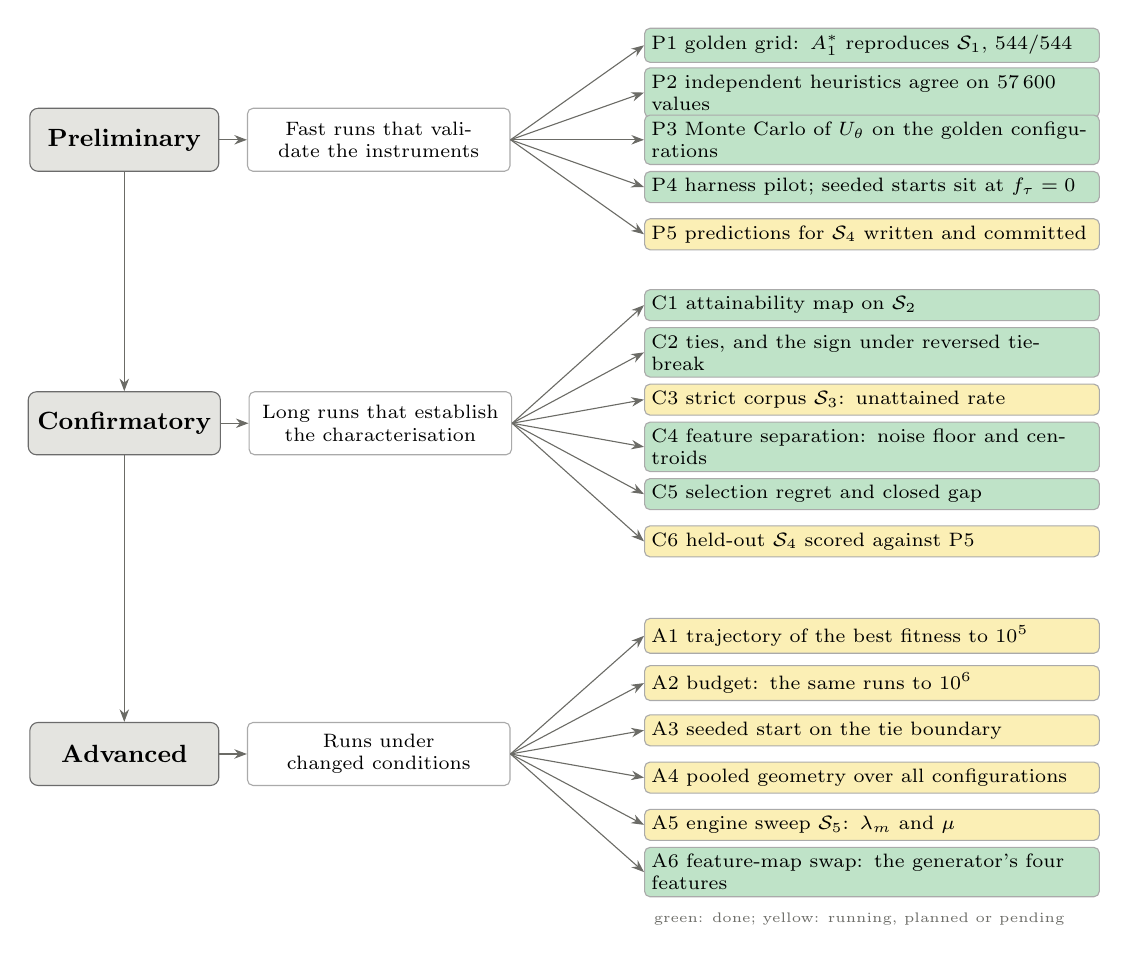
\begin{tikzpicture}[
  every node/.style={font=\scriptsize, align=center},
  ph/.style={draw=ink!70, fill=pGray, rounded corners=3pt, minimum width=2.4cm, minimum height=0.8cm, font=\small\bfseries},
  what/.style={draw=ink!40, fill=white, rounded corners=2pt, text width=3.1cm, minimum height=0.8cm},
  run/.style={draw=ink!40, fill=#1, rounded corners=2pt, text width=5.6cm, inner sep=2.5pt, anchor=west, align=left},
  arr/.style={-{Stealth[length=1.6mm]}, color=inkSoft}]
\node[ph] (p) at (0,0) {Preliminary};
\node[ph] (c) at (0,-3.6) {Confirmatory};
\node[ph] (a) at (0,-7.8) {Advanced};
\draw[arr] (p) -- (c); \draw[arr] (c) -- (a);
\node[what, right=0.35cm of p] (pw) {Fast runs that validate the instruments};
\node[what, right=0.35cm of c] (cw) {Long runs that establish the characterisation};
\node[what, right=0.35cm of a] (aw) {Runs under changed conditions};
\draw[arr] (p) -- (pw); \draw[arr] (c) -- (cw); \draw[arr] (a) -- (aw);
\foreach \y/\col/\txt in {
  1.2/pGreen/{P1 golden grid: $\Astar$ reproduces $\mathcal S_1$, $544/544$},
  0.6/pGreen/{P2 independent heuristics agree on $57\,600$ values},
  0.0/pGreen/{P3 Monte Carlo of $\Utheta$ on the golden configurations},
  -0.6/pGreen/{P4 harness pilot; seeded starts sit at $f_\tau=0$},
  -1.2/pYellow/{P5 predictions for $\mathcal S_4$ written and committed}}{
  \node[run=\col] (n) at (6.6,\y) {\txt}; \draw[arr] (pw.east) -- (n.west);}
\foreach \y/\col/\txt in {
  -2.1/pGreen/{C1 attainability map on $\mathcal S_2$},
  -2.7/pGreen/{C2 ties, and the sign under reversed tie-break},
  -3.3/pYellow/{C3 strict corpus $\mathcal S_3$: unattained rate},
  -3.9/pGreen/{C4 feature separation: noise floor and centroids},
  -4.5/pGreen/{C5 selection regret and closed gap},
  -5.1/pYellow/{C6 held-out $\mathcal S_4$ scored against P5}}{
  \node[run=\col] (n) at (6.6,\y) {\txt}; \draw[arr] (cw.east) -- (n.west);}
\foreach \y/\col/\txt in {
  -6.3/pYellow/{A1 trajectory of the best fitness to $10^{5}$},
  -6.9/pYellow/{A2 budget: the same runs to $10^{6}$},
  -7.5/pYellow/{A3 seeded start on the tie boundary},
  -8.1/pYellow/{A4 pooled geometry over all configurations},
  -8.7/pYellow/{A5 engine sweep $\mathcal S_5$: $\lambda_m$ and $\mu$},
  -9.3/pGreen/{A6 feature-map swap: the generator's four features}}{
  \node[run=\col] (n) at (6.6,\y) {\txt}; \draw[arr] (aw.east) -- (n.west);}
\node[font=\tiny, text=inkSoft, anchor=west] at (6.6,-9.9) {green: done; yellow: running, planned or pending};
\end{tikzpicture}
\captionof{figure}{Experimental methodology. Each phase feeds the next: the instruments
validated in the first are the ones the second measures with, the predictions written in the
first are scored in the second, and the third reuses the second's cells under changed
conditions.}\label{fig:phases}
\end{center}

\begin{definition}[Experimental plan]\label{def:plan}
Each experiment is a tuple (instance set, metric, hypothesis decided, status).
\begin{center}\scriptsize
\begin{tabular}{@{}llp{3.1cm}p{2.6cm}p{2.0cm}p{2.2cm}@{}}
\toprule
& Experiment & Set & Metric & Decides & Status \\
\midrule
P1 & Output identity & $\mathcal S_1$ & (i) & Def.~\ref{def:states} & done, $544/544$ \\
P2 & Heuristic agreement & $\mathcal S_2$ & (ii), recomputed vs.\ native & instrument & done, $0$ mismatches \\
P3 & Uniform baseline & $\Utheta$ at $\theta_0$--$\theta_3$ & (ii) on $\Utheta$ & context & done \\
P4 & Harness pilot & $n{=}50$, 16 runs & (vii); $f_\tau=0$ at start & instrument & done \\
P5 & Preregistration & predictions for $\mathcal S_4$ & all & H\ref{h:selection}--H\ref{h:pca} & written; commit pending \\
\addlinespace[2pt]
C1 & Attainability map & $\mathcal S_2$ & (ii), (iii) per cell & H\ref{h:map} & done \\
C2 & Ties & $\mathcal S_2$ & (iv); sign under reversed tie-break & H\ref{h:sign} & done \\
C3 & Strict corpus & $\mathcal S_3$ & (ii): $\hat u_C$ & H\ref{h:map} & running \\
C4 & Feature separation & $\mathcal S_2$, all and strict & (v) per cell & H\ref{h:pca} & done \\
C5 & Selection & $\mathcal S_2$ & (vi) per cell and per $n$ & H\ref{h:selection} & done \\
C6 & Held-out test & $\mathcal S_4$ & as P5 & H\ref{h:selection}--H\ref{h:pca} & after P5 \\
\addlinespace[2pt]
A1 & Trajectory & $n\in\{100,\dots,1000\}$, $b{=}10$, $\alpha{=}0.25$, bounded types, $5$ seeds & (vii) to $10^{5}$ & H\ref{h:budget} & running \\
A2 & Budget $\times10$ & same runs & (vii) to $10^{6}$ & H\ref{h:budget} & running \\
A3 & Seeded start & same cells & (vii), seeded & H\ref{h:budget} & running \\
A4 & Pooled geometry & $\mathcal S_2$ & (v) pooled & descriptive & done \\
A5 & Engine sweep & $\mathcal S_5$ & (ii), (v), (vi) & reach of H\ref{h:selection}--H\ref{h:pca} & planned \\
A6 & Feature-map swap & $\mathcal S_2$, four generator features & (v), (vi) & H\ref{h:pca} & done \\
\bottomrule
\end{tabular}
\end{center}
\end{definition}

\begin{remark}[Decision rules and statistical resolution]
Each hypothesis is decided by the refutation condition it states, applied first in-sample and
then, without change, to $\mathcal S_4$. Hypotheses are aggregate statements over many cells;
per-cell tables are descriptive and carry no per-cell significance claims, so no correction
for multiple comparisons is applied to them. A cell of $60$ instances has an exact
Clopper--Pearson half-width of at most $0.13$ for $q$ near $\tfrac12$, bounds $q<0.049$ when
$\hat q=0$ and $q>0.951$ when $\hat q=1$ (one-sided, $95\%$). A5 does not decide a hypothesis
by itself: it reports whether each refutation condition still holds at the other engine
settings, and a hypothesis that fails there is restricted to the campaign setting in the
support boundary.
\end{remark}

\subsection{Preregistered held-out test}\label{sec:prereg}

\begin{plain}{why this exists}
Several thresholds above were written after looking at the campaign's results. A committee
can fairly say that such a hypothesis was fitted to the data. The answer is to predict cells
the analysis has never seen, write the predictions down, commit them with a timestamp, and
only then generate those cells. The predictions below are interpolations of the campaign plus
the bound, and they are scored with the scripts already in the repository.
\end{plain}

\begin{definition}[Predictions for $\mathcal S_4$]\label{def:prereg}
On $\mathcal S_4$ ($n\in\{300,700\}$, $b=12$, $\alpha\in\{0.15,0.40\}$, $60$ instances per cell):
\begin{enumerate}[label=\textbf{R\arabic*},leftmargin=2.6em,itemsep=2pt]
\item (Corollary~\ref{cor:regret}, implementation check) $\max_I r(I)/2^{\bp}<1$.
\item (H\ref{h:map}a) each unbounded type has at least $59$ strict instances in each of the four cells.
\item (H\ref{h:map}b) for each bounded type and each $\alpha$, strict$(n{=}700)\le$ strict$(n{=}300)+6$.
\item (H\ref{h:map}c) \DEF-\textsc{easy}, \MAXP-\textsc{easy} and \MAXPW-\textsc{hard} have at most $6$ strict instances in both cells with $n=700$; no numeric prediction is made for \MINW-\textsc{easy}.
\item (H\ref{h:selection}) $\bar r_C<1\%$ in all four cells and $\bar r_C<0.1\%$ in both cells with $n=700$.
\item (H\ref{h:pca}a) $\sqrt n\cdot w_C\in[0.26,0.40]$ and $w_C/w^{U}_{n,12}\in[0.80,1.20]$ in all four cells.
\item (H\ref{h:pca}b) $d_C(n{=}700)\le1.10\,d_C(n{=}300)$ for both $\alpha$.
\end{enumerate}
Each prediction is reported as met or not met; none is revised after generation. The commit
that contains this definition is recorded in Appendix~D before $\mathcal S_4$ is generated.
\end{definition}

% =====================================================================
\section{Campaign design of $\mathcal S_2$ and $\mathcal S_3$}\label{sec:design}

\begin{center}\small
\begin{tabular}{@{}lp{4.4cm}p{7.4cm}@{}}
\toprule
Axis & Levels & Note \\
\midrule
$n$ & $50,\ 100,\ 200,\ 500,\ 1000$ & item count; $L=2nb$ \\
$\bw=\bp=b$ & $10,\ 14$ & $\Wmax=\Pmax=2^{b}$, so the declared box is exact \\
$\alpha$ & $0.05,\ 0.25,\ 0.50$ & $c=\lfloor\alpha\,n\,(2^{b}+1)/2\rfloor$, the expected total weight under $\Utheta$ times $\alpha$ \\
$\tau$ & the $8$ labelled types & \\
$\lambda_m$ & $11$ & expected flips per offspring; $p_m=\lambda_m/L$ \\
$\mu,\ p_c,\ k$ & $10,\ 0.8,\ 3$ & $\mu$ even, so $\mu'=\mu$ \\
seeds & $30$ per cell; shared across $\alpha$ within $(n,b)$ & $2$ instances per call: $60$ per $(\theta,\tau)$ \\
\bottomrule
\end{tabular}
\end{center}

Thirty configurations, eight types, $14\,400$ instances: \code{runs/pisinger_main}. The
mutation axis is parametrised by $\lambda_m$ rather than $p_m$ so that a level means the
same number of expected flips at $L=1\,000$ and at $L=28\,000$; $\lambda_m=11$ is the
regime of the shipped $p_m=0.1$ at the default configuration ($L=110$), not at the
campaign's lengths, and it is held fixed here; its reach is tested by A5. The capacity rule fixes
$\alpha$ nominally; the realised $\alpha=c/\sum w$ is recorded per instance. The same
design is being rerun with \code{--require-strict} ($r_{\max}=10$) to measure unattained
rates directly (\code{runs/pisinger_strict}, $976$ of $14\,400$ instances done, $196$
unattained, all in the four bounded types) \pending.

\paragraph{Instruments.} Every measurement is recomputed from the emitted \code{.kp} files
by an implementation of the four heuristics independent of the generator (a stable sort by
key and one first-fit pass); on the $57\,600$ heuristic values of the campaign it agrees with
the generator's own values exactly \evid{V3}. The feature map is that of the 2019 paper,
$\Phi(I)=(\bar{\hat w},\operatorname{med}\hat w,\operatorname{sd}\hat w,\bar{\hat p},
\operatorname{med}\hat p,\operatorname{sd}\hat p,\tfrac12(\rho+1))\in[0,1]^{7}$ with
$\hat w=w/\max w$, $\hat p=p/\max p$, $\operatorname{sd}$ with divisor $n-1$.

% =====================================================================
\section{Results measured so far}\label{sec:results}

\subsection{Outcome of the label per type}

\begin{center}\small
\begin{tabular}{@{}lrrrp{6.2cm}@{}}
\toprule
Type & strict & tie & failed & where the failures are \\
\midrule
\DEF-\textsc{easy}   & $867$  & $0$   & $933$  & three at $n=100$, then $n\ge200$; $100\%$ at $n\ge500$ \\
\DEF-\textsc{hard}   & $1800$ & $0$   & $0$    & \\
\MAXP-\textsc{easy}  & $1088$ & $0$   & $712$  & $n\ge500$, all $\alpha$ \\
\MAXP-\textsc{hard}  & $1800$ & $0$   & $0$    & \\
\MAXPW-\textsc{easy} & $1800$ & $0$   & $0$    & \\
\MAXPW-\textsc{hard} & $274$  & $203$ & $1323$ & failed at $\alpha\le0.25$ from $n=50$, and at $n\ge500$ for every $\alpha$; ties at $\alpha=0.5$, $n\le200$ \\
\MINW-\textsc{easy}  & $1289$ & $3$   & $508$  & $n\ge500$, mostly $\alpha\le0.25$ \\
\MINW-\textsc{hard}  & $1800$ & $0$   & $0$    & \\
\midrule
total & $10\,718$ & $206$ & $3\,476$ & \\
\bottomrule
\end{tabular}
\end{center}

The four types with no failure are exactly the four Corollary~\ref{cor:window} leaves
unbounded; the four with failures are exactly the bounded ones. In every failed
\textsc{easy} instance the actual winner is \MAXPW\ ($933/933$, $712/712$, $508/508$); in
$1\,224$ of the $1\,323$ failed \MAXPW-\textsc{hard} instances \MAXPW\ is the actual winner
\evid{V3}. The unbounded types have $60/60$ strict in each of their $120$ cells ($q>0.951$
each); $\hat q=0$ in $47$ of the $120$ cells of the bounded types ($q<0.049$ each). This is the
measured attainability map; the per-cell table is \code{runs/pisinger_main/ties/ties.csv} and
the figure \code{outcomes_per_cell.png}. Strict counts of the bounded types per $(b,\alpha)$
never increase with $n$; they are not ordered in $\alpha$ (Hypothesis~\ref{h:map}).

\subsection{Ties}\label{sec:ties-results}

\begin{itemize}[leftmargin=1.6em,itemsep=2pt]
\item \emph{Target ties:} $206$; $203$ in \MAXPW-\textsc{hard}, all but four at $\alpha=0.5$,
$n\le200$ (per cell up to $51$ of $60$); in $117$ of them the four heuristics reach the
same profit. Three in \MINW-\textsc{easy}.
\item \emph{Pair ties:} $1\,014$ instances ($7.0\%$) with fewer than four distinct profits
($1$ distinct: $117$; $2$: $167$; $3$: $730$); $218$ involve the target, $796$ do not. All
at $n\le200$ except three at $n=1000$; none at $n=500$. The most frequent pair is
$\MAXPW=\MINW$ ($617$). The heuristics that never tie among themselves in the unbounded
types are recorded in the pair-by-type matrix (\code{ties_all.png}).
\item \emph{Order ties:} $1\,962$ instances ($13.6\%$) in which reversing the index tie-break
changes at least one heuristic's profit: \MAXP\ $1\,095$, \MINW\ $1\,142$, \MAXPW\ $9$.
$1\,799$ at $b=10$ against $163$ at $b=14$; $71$ at $n=50$ rising to $922$ at $n=1000$.
\item \emph{Sign under order ties:} $40$ instances ($0.28\%$; $38$ at $b=10$, $0.53\%$ of
that half) change the sign of $f_\tau$ when the tie-break is reversed: \MINW-\textsc{easy}
$17$, \MAXPW-\textsc{hard} $12$, \MAXP-\textsc{easy} $11$. In all $40$ the shipped
tie-break gives $f_\tau\ge0$ and the reverse gives $f_\tau<0$. Hypothesis~\ref{h:sign} is
refuted at its $1\%$ threshold \evid{V3}.
\end{itemize}
The where and when of ties (small $n$, loose knapsack, low $b$) is descriptive: the first
two follow from the $k=n$ case of Proposition~\ref{prop:bound} and from the improbability of
equal sums at large $n$, the third from the pigeonhole principle, and none was posed as a
hypothesis.

\subsection{Value of selection}\label{sec:selection}

\begin{plain}{what the table says}
If someone had to pick one heuristic for every instance of the corpus, \MAXPW\ is the
pick. The table asks how much a perfect selector, one that knows the best heuristic for
every instance, would gain over that pick. At $n=50$ with a tight knapsack the answer is
about $6\%$ of the profit on average, with individual instances up to $24\%$; from $n=200$ it
is under $1\%$ on average, and at $n=1000$ it is exactly zero except with the tightest
knapsack. A selector trained on the features recovers part of that, but part of very little.
\end{plain}

Per cell of $\mathcal S_2$ (both $b$ pooled, since the two agree within $0.6$ points):

\begin{center}\small
\begin{tabular}{@{}lccccc@{}}
\toprule
& $n=50$ & $n=100$ & $n=200$ & $n=500$ & $n=1000$ \\
\midrule
share of instances with $r(I)>0$, $\alpha=0.05$ & $56\%$ & $46\%$ & $37\%$ & $13\%$ & $9\%$ \\
\quad $\alpha=0.25$ & $49\%$ & $38\%$ & $24\%$ & $1\%$ & $0\%$ \\
\quad $\alpha=0.50$ & $54\%$ & $48\%$ & $32\%$ & $1\%$ & $0\%$ \\
mean relative regret, $\alpha=0.05$ & $6.5\%$ & $2.1\%$ & $0.62\%$ & $0.074\%$ & $0.007\%$ \\
\quad $\alpha=0.25$ & $1.4\%$ & $0.41\%$ & $0.094\%$ & $0.0002\%$ & $0$ \\
\quad $\alpha=0.50$ & $0.75\%$ & $0.24\%$ & $0.046\%$ & $0.0001\%$ & $0$ \\
maximum relative regret, $\alpha=0.05$ & $24\%$ & $10\%$ & $2.7\%$ & $0.8\%$ & $0.3\%$ \\
\MAXPW\ is the oracle's choice & $47\%$ & $56\%$ & $69\%$ & $95\%$ & $97\%$ \\
\bottomrule
\end{tabular}
\end{center}

The maximum of $r(I)/2^{\bp}$ over the corpus is $0.965$, as Corollary~\ref{cor:regret}
requires. Restricted to strict instances the mean relative regret is
$3.0\%,\ 1.0\%,\ 0.31\%,\ 0.05\%,\ 0.00\%$ for $n=50$ to $1000$. No cell with $n\ge200$
reaches $1\%$; Hypothesis~\ref{h:selection} is supported in-sample \evid{V3}
(\code{runs/pisinger_main/selection_regret.csv}).

Trained selectors, per $n$ over all cells (\code{runs/pisinger_main/selection_gap.csv}):

\begin{center}\small
\begin{tabular}{@{}lccccc@{}}
\toprule
& $n=50$ & $n=100$ & $n=200$ & $n=500$ & $n=1000$ \\
\midrule
mean relative regret of \MAXPW\ & $2.86\%$ & $0.91\%$ & $0.25\%$ & $0.02\%$ & $0.002\%$ \\
cost-sensitive selector on $\Phi$ & $2.11\%$ & $0.69\%$ & $0.16\%$ & $0.01\%$ & $0.001\%$ \\
\quad closed gap & $25\%$ & $34\%$ & $45\%$ & $51\%$ & $85\%$ \\
\quad accuracy (picks an oracle heuristic) & $66\%$ & $70\%$ & $81\%$ & $97\%$ & $99\%$ \\
plain classifier: accuracy & $76\%$ & $86\%$ & $93\%$ & $98\%$ & $99\%$ \\
\quad closed gap & $-9\%$ & $-91\%$ & $-110\%$ & $1\%$ & $82\%$ \\
same selector on the four generator features: closed gap & $32\%$ & $23\%$ & $27\%$ & $22\%$ & $86\%$ \\
\bottomrule
\end{tabular}
\end{center}

Two readings. A selector trained on the features closes a quarter to a half of the gap at
$n\le500$, so the features carry information about which heuristic wins; but the gap it
closes is $0.75$ percentage points of profit at $n=50$ and $0.09$ at $n=200$, and a
closed gap of $85\%$ at $n=1000$ is $85\%$ of $0.002\%$. And accuracy is the wrong score for
this question: the classifier picks an oracle heuristic more often than the cost-sensitive
selector and still loses profit against always choosing \MAXPW, because when it is wrong it is
wrong by a lot. The configuration used to tune the 2019 generator ($n=40$, $\Pmax=100$, so
$\bp=7$) lies in the corner of the table where the window is a visible fraction of the value;
whether the corpora of that study behave as $\mathcal S_2$ does at $n=50$ is not measured
here.

\subsection{Geometry in feature space}\label{sec:pca}

\begin{plain}{what changes with $n$, and what does not}
With few items the instances of different types overlap in feature space; with many items
they form clean clusters. It is tempting to read that as the generator tailoring instances
more sharply at large $n$. It is not. Each feature is an average or a spread over $n$ items,
so its random fluctuation shrinks like $1/\sqrt n$, exactly as it does for instances drawn at
random with no tailoring at all. Meanwhile the distance between the centres of the type
clusters does not grow; it shrinks. The clusters sharpen because the noise falls faster than
the signal, and that is a property of the feature map, not of the generator.
\end{plain}

Signal and noise per $n$, averaged over the six $(b,\alpha)$ cells
(\code{runs/pisinger_main/pca/separation.csv}):

\begin{center}\small
\begin{tabular}{@{}llccccc@{}}
\toprule
& & $n=50$ & $n=100$ & $n=200$ & $n=500$ & $n=1000$ \\
\midrule
all instances & within-type spread $w_C$ & $0.042$ & $0.031$ & $0.023$ & $0.015$ & $0.011$ \\
& noise floor $w^{U}$ (uniform instances) & $0.047$ & $0.033$ & $0.024$ & $0.015$ & $0.011$ \\
& $\sqrt n\,w_C$ & $0.30$ & $0.31$ & $0.32$ & $0.34$ & $0.34$ \\
& between-type distance $d_C$ & $0.358$ & $0.330$ & $0.298$ & $0.251$ & $0.227$ \\
& silhouette by type & $0.27$ & $0.36$ & $0.43$ & $0.47$ & $0.54$ \\
& silhouette by heuristic & $0.04$ & $0.06$ & $0.07$ & $0.06$ & $0.06$ \\
\addlinespace[2pt]
strict instances & types with $\ge5$ instances & $7.8$ & $7.3$ & $7.0$ & $4.8$ & $4.3$ \\
& $d_C$ & $0.361$ & $0.336$ & $0.313$ & $0.290$ & $0.265$ \\
& silhouette by type & $0.28$ & $0.39$ & $0.50$ & $0.64$ & $0.69$ \\
& silhouette by heuristic & $0.05$ & $0.10$ & $0.19$ & $0.57$ & $0.64$ \\
\bottomrule
\end{tabular}
\end{center}

Per cell, $w_C/w^{U}\in[0.82,1.06]$, $\sqrt n\,w_C\in[0.28,0.35]$, and $d_C$ never rises from
one $n$ to the next, ending at $45$--$85\%$ of its value at $n=50$, on all instances and on
strict ones. With the generator's own four features the pattern is the same:
$\sqrt n\,w_C=0.33$ to $0.32$ and $d_C$ from $0.24$ to $0.17$, while the silhouette by type
rises from $0.17$ to $0.26$. Hypothesis~\ref{h:pca} is supported in-sample \evid{V3}.

\paragraph{Descriptive, with caveats.} On all instances the silhouette by heuristic stays at
$0.04$--$0.07$: within a configuration the \textsc{easy} and \textsc{hard} instances of one
heuristic lie in different regions. On strict instances the silhouette by heuristic jumps to
$0.57$--$0.64$ at $n\ge500$; that is a composition effect, not a finding, because at those
sizes the bounded types have almost no strict instances and the remaining four or five types
are nearly one per heuristic, so ``type'' and ``heuristic'' become the same label. Pooled over
the thirty configurations the silhouette by type is $0.15$ (PC1 $55\%$, PC2 $17\%$); since
$\Phi$ contains neither $n$ nor $\alpha$, pooling is expected to blur the clusters and is not
posed as a hypothesis. PC1 opposes the profit moments to the weight moments (loadings $+0.45$,
$+0.44$ on $\bar{\hat p}$, $\operatorname{med}\hat p$; $-0.42$, $-0.42$ on $\bar{\hat w}$,
$\operatorname{med}\hat w$; $-0.30$ on the correlation) and PC2 is dominated by
$\operatorname{sd}\hat p$ ($+0.67$). The insensitivity to $b$ is expected, since $\Phi$ is
normalised per instance.

% =====================================================================
\section{Diagnostic experiments}\label{sec:experiments}

Run on the engine of $\Astar$ (same classes, same seed tree; the budget literal and the
initial population are the only things the harness controls), for the four bounded types,
$n\in\{100,200,500,1000\}$, $b=10$, $\alpha=0.25$, five seeds, the campaign's engine
parameters. Results \pending; the design and the decision rules of
Hypothesis~\ref{h:budget} were fixed before the runs finished.

\begin{enumerate}[label=\textbf{E\arabic*},leftmargin=3em,itemsep=3pt]
\item \emph{Trajectory.} The best fitness against evaluations at log-spaced checkpoints up
to $\Emax$; up to $\Emax$ this is the campaign's run. \emph{Reads:} whether the elite is still
improving at $\Emax$ (budget) or stalled below $0$ (structure).
\item \emph{Budget.} The same runs continued to $10^{6}$ evaluations, which is
$\Emax\cdot n/100$ at $n=1000$. \emph{Decision:} as stated in Hypothesis~\ref{h:budget}(a).
\item \emph{Seeded start.} The initial population is placed on the tie boundary
($f_\tau=0$ exactly: items stored in ratio order for \DEF-\textsc{easy}; equal weights for
\MAXP-\textsc{easy}; equal profits for \MINW-\textsc{easy}; equal weights and profits for
\MAXPW-\textsc{hard}) and evolved with the same operators and budget. \emph{Reads:} whether
the search can step from $0$ into $W_\tau$ when the alignment problem of
Remark~\ref{rem:window} is solved for it. A seeded run that reaches $f_\tau>0$ shows that
strict instances exist and are one step away; a seeded run that stays at $0$ shows that the
operators leave the boundary in the wrong direction.
\end{enumerate}

The one caveat: the seeded point for \MAXPW-\textsc{hard} is the degenerate instance in which
the four heuristics coincide; failure to leave it does not show that strict
\MAXPW-\textsc{hard} instances do not exist.

% =====================================================================
\section{Threats to validity and design responses}\label{sec:threats}

\begin{plain}{what this section is}
Every objection a committee could reasonably raise against the hypotheses, the design or the
reading of the results, each paired with what the design does about it and where. Where the
design cannot remove an objection, the claim is restricted instead, and the support boundary
says so.
\end{plain}

\begin{center}\scriptsize
\begin{longtable}{@{}p{0.6cm}p{4.6cm}p{6.8cm}p{2.2cm}@{}}
\toprule
& Objection & Design response & Where \\
\midrule
\endhead
\multicolumn{4}{@{}l}{\emph{Construct validity: are the right things measured?}} \\
T1 & ``Hard'' suggests hard to solve. & \textsc{hard} names an objective only; solver hardness is never claimed; Prop.~\ref{prop:factor} shows no hardness term. & Def.~\ref{def:labelled}, Sec.~\ref{sec:support} \\
T2 & The value of selection is judged against \MAXPW; another baseline would show large gains. & The single best solver is the standard baseline of algorithm selection; the text reports that against any fixed non-\MAXPW\ choice selection pays $22$--$92\%$. & Remark after Cor.~\ref{cor:regret} \\
T3 & Four greedy heuristics are a toy portfolio; hyper-heuristics combine them during construction. & Cor.~\ref{cor:regret}(ii) holds for every feasible packing, including hyper-heuristics and exact solvers. & Cor.~\ref{cor:regret} \\
T4 & Relative regret hides absolute profit that may matter. & Both are reported; the absolute bound is $2^{\bp}$ per instance. & metric (vi) \\
T5 & A selector that scores well on accuracy was not tried, or a weak one was. & A cost-sensitive random forest with grouped cross-validation is used; a classifier is shown to illustrate why accuracy misleads. & Sec.~\ref{sec:selection} \\
T6 & The seven features are the static use of the paper's dynamic features; the generator exposes different ones. & A6 repeats the separation and the selector with the generator's four features; the conclusions do not change. & Sec.~\ref{sec:pca}, \ref{sec:selection} \\
T7 & Silhouettes grow with $n$ for reasons unrelated to the generator. & H\ref{h:pca} is stated on the noise floor and the centroid distance, not on the silhouette. & H\ref{h:pca} \\
T8 & Failed instances appear in the feature analysis under a label they do not have. & Every feature result is repeated on strict instances; the composition effect at $n\ge500$ is reported. & Sec.~\ref{sec:pca} \\
\addlinespace[3pt]
\multicolumn{4}{@{}l}{\emph{Internal validity: could the results be artefacts of the pipeline?}} \\
T9 & The analysis code may disagree with the generator. & All $57\,600$ heuristic values are recomputed independently and agree; $\Astar$ reproduces the golden grid byte for byte. & P1, P2 \\
T10 & Instances of one call are not independent, and seeds are reused. & The two instances of a call are independent runs; cross-validation groups by call; seeds are shared only across $\alpha$ within $(n,b)$, and the text says so. & Def.~\ref{def:sets} \\
T11 & The diagnostic harness is not the generator. & It builds the engine from the generator's own classes as \code{KP.evolve} does; up to $10^{5}$ evaluations a random-start run is the campaign's run. & Sec.~\ref{sec:experiments} \\
T12 & The label depends on how ties among items are broken. & Measured: the sign changes in $0.28\%$ of instances (H\ref{h:sign}). & C2 \\
\addlinespace[3pt]
\multicolumn{4}{@{}l}{\emph{Statistical conclusion validity}} \\
T13 & $60$ instances per cell is too few. & Exact Clopper--Pearson bounds are reported; $\hat q=0$ means $q<0.049$ and $\hat q=1$ means $q>0.951$. & Remark on decision rules \\
T14 & $240$ cells invite false discoveries. & Hypotheses are aggregate; per-cell tables are descriptive and carry no significance claims. & Remark on decision rules \\
T15 & Hypotheses and thresholds were fitted to the data (HARKing). & Thresholds fixed afterwards are marked; the four empirical hypotheses are re-tested on a preregistered held-out design with predictions committed before generation; H\ref{h:sign}'s threshold was set before measuring and the hypothesis was refuted. & Sec.~\ref{sec:prereg} \\
\addlinespace[3pt]
\multicolumn{4}{@{}l}{\emph{External validity: how far do the results reach?}} \\
T16 & The results hold only at $\mu=10$, $\lambda_m=11$, $k=3$, $p_c=0.8$. & Exact claims do not depend on the engine; empirical claims are labelled with their setting and re-tested at $\lambda_m\in\{3,33\}$ and $\mu=30$. & Sec.~1, A5 \\
T17 & $\lambda_m=11$ is not the shipped $p_m=0.1$ at large $L$. & Stated explicitly; the shipped literal would apply $2\,000$ flips per offspring at $L=20\,000$, a random-search regime; the campaign studies a fixed search regime instead. & Sec.~1, Sec.~\ref{sec:design} \\
T18 & Thirty configurations do not cover the space. & Held-out $n$, $b$ and $\alpha$ levels in $\mathcal S_4$. & C6 \\
T19 & $\bw=\bp$ throughout. & The bound depends on $\bp$ only; a design with $\bw\ne\bp$ needs a driver change and is recorded as a limitation. & Sec.~\ref{sec:support} \\
T20 & Profits that scale with $n$ would escape the bound. & True; H\ref{h:selection} is restricted to a fixed profit range, and the support boundary says so. & H\ref{h:selection} \\
T21 & The budget experiment covers few cells and seeds. & H\ref{h:budget} is stated for exactly those cells and budgets. & H\ref{h:budget} \\
T22 & The 2019 study used other configurations. & No claim is made about its corpora; only the position of its tuning configuration in the regret table is noted. & Sec.~\ref{sec:selection} \\
\bottomrule
\end{longtable}
\end{center}

% =====================================================================
\section{Support boundary (to be completed)}\label{sec:support}

The last chapter is a table with one row per claim a user of the generator might make; each
row cites the proposition or the cell that decides it. Rows fixed by what is proved and
measured so far:

\begin{center}\small
\begin{tabular}{@{}p{6.4cm}p{2.2cm}p{6.6cm}@{}}
\toprule
Claim & Status & Decided by \\
\midrule
The interface bounds $\Wmax,\Pmax$ describe the emitted coefficients & not supported & Prop.~\ref{prop:reach}, \ref{prop:dyadic}; $51.5\%$ overshoot at the defaults \\
Every emitted $h$-\textsc{easy} file has $h$ as its best heuristic & not supported & $3\,476$ failed of $14\,400$; $q_{\theta,\tau}=0$ in $47$ of the $240$ cells \\
The four \textsc{hard} types of \DEF, \MAXP, \MINW\ and \MAXPW-\textsc{easy} are reliably delivered on the design & supported & $1\,800/1\,800$ each \\
A corpus filtered by \code{--require-strict} is a sample of $\Gtt$ & not supported; it is a sample of $\Gtt(\cdot\mid W_\tau)$ & Prop.~\ref{prop:conditional} \\
Margins of the bounded types can be made large by a longer search & not supported & Prop.~\ref{prop:bound}: $f_\tau<2^{\bp}$ \\
``Hard'' instances are hard for an exact solver & not supported & Prop.~\ref{prop:factor}: no hardness term in $f_\tau$ \\
Algorithm selection over $\heur$ pays on this corpus & supported at $n\le100$ in relative terms ($0.9$--$2.9\%$ mean, a trained selector recovering a quarter to a third); not supported at $n\ge200$ & Cor.~\ref{cor:regret}; H\ref{h:selection}; Sec.~\ref{sec:selection} \\
Any algorithm, with profits in $\{1,\dots,2^{\bp}\}$, gains $2^{\bp}$ or more over \MAXPW\ on some instance & not supported, exactly & Cor.~\ref{cor:regret}(ii) \\
A generator whose profit range grows with $n$ is bound the same way & not addressed & outside the scope (T20) \\
Within a configuration the types occupy distinct regions of $\Phi$ & supported, with overlaps listed & Sec.~\ref{sec:pca} \\
The generator tailors instances more distinctly at larger $n$ & not supported; the sharper clusters are the $n^{-1/2}$ concentration of $\Phi$ & H\ref{h:pca} \\
The types are separable in $\Phi$ across configurations & not supported & pooled silhouette $0.15$ \\
The empirical results hold at other engine settings & \pending & A5 \\
The empirical results predict unseen configurations & \pending & C6 \\
Results with $\bw\ne\bp$ & not addressed & limitation (T19) \\
The label is a property of the item multiset & supported up to $0.5\%$ & order ties change a value in $13.6\%$ of instances and the sign in $0.28\%$ (H\ref{h:sign}) \\
The failure at large $n$ is a budget artefact & \pending & E1--E3 \\
\bottomrule
\end{tabular}
\end{center}

% =====================================================================
\section{Thesis outline}\label{sec:outline}

One claim per chapter; every figure carries the number that decides it in its title.

\begin{enumerate}[label=\textbf{Ch.~\arabic*},leftmargin=3.6em,itemsep=4pt]
\item \textbf{Introduction and object of study.} The 2019 generator and its use in later
hyper-heuristic work; why an evolutionary generator is a sampler whose law must be
characterised; Definitions~\ref{def:states} and~\ref{def:object}; \ref{rq:what}--\ref{rq:support};
the hypotheses; the scope (Section~1 of this document).
\item \textbf{The artefact.} $\Aone$ and $\Astar$; the six changes and the golden grid;
Propositions~\ref{prop:reach}--\ref{prop:budget}; the strict driver and
Proposition~\ref{prop:conditional}. \emph{From Revision 12:} Sections 2, 5, 6, 7.1--7.3, 9,
11, 13 compressed; source boxes, class diagram, cost model, chromosome trace and the Latin
hypercube analysis go to Appendices A--C.
\item \textbf{Geometry of the objective.} Proposition~\ref{prop:bound},
Corollary~\ref{cor:window}, Corollary~\ref{cor:regret} and its reading for algorithm
selection, Remark~\ref{rem:window}, Definition~\ref{def:ties}; the predicted attainability
map as a table over the design. \emph{New.}
\item \textbf{Methodology and the characterisation campaign.} Instance sets, metrics and
phases (Section~\ref{sec:method}, in the format of the institutional template: 3.1
instances, 3.2 metrics, Figure~\ref{fig:phases}); design (Section~\ref{sec:design}); the measured
map against the predicted one (figure \code{outcomes_per_cell}); ties
(\code{pair_ties_per_cell}, \code{ties_all}); the strict campaign's unattained rates;
the selection-regret table (Section~\ref{sec:selection});
feature-space geometry with its signal/noise split (Section~\ref{sec:pca}); the
preregistered held-out test (Section~\ref{sec:prereg}). \emph{From today's analyses and the
notebook's feature map.}
\item \textbf{Diagnosis, robustness and support boundary.} A1--A3 and the decision on
Hypothesis~\ref{h:budget}; the engine sweep A5 and the feature-map swap A6; threats to
validity (Section~\ref{sec:threats}); the support-boundary table; conclusions.
\end{enumerate}

\paragraph{Appendices.}
A: source boxes and line references for every proposition (Revision 12, Sections 3--9).
B: the golden-file kit and the verification record.
C: the Latin hypercube analysis of the 2019 tuning design and the effective-parameter map.
D: reproducibility: \code{tools/characterise.py}, \code{tools/pca_feat7.py},
\code{tools/ties_plot.py}, \code{tools/order_tie_sign.py}, \code{tools/selection_gap.py},
\code{tools/feature_separation.py}, \code{tools/feature4_robustness.py},
\code{tools/experiments/}, the notebook, seeds and command lines, and the commit hash of the
preregistration of Definition~\ref{def:prereg}.


% =====================================================================
\section*{Vocabulary}
\addcontentsline{toc}{section}{Vocabulary}
\begin{small}
\begin{tabular}{@{}p{3.4cm}p{11.6cm}@{}}
\toprule
strict / tie / failed & the outcome of one emitted instance: $f_\tau(\beta)>0$, $=0$, $<0$ \\
$q_{\theta,\tau}$ & probability that a run is strict; the attainability map is $q$ over the design \\
attainable / reliable cell & $q>0$ / $q=1$ within resolution \\
unattained & an instance the strict driver gave up on after $r_{\max}+1$ runs \\
bounded / unbounded type & whether Corollary~\ref{cor:window} caps $f_\tau$ below $2^{\bp}$ \\
target tie / pair tie / order tie & Definition~\ref{def:ties} \\
$\Phi$ & the seven-feature map of the 2019 paper, computed once per instance \\
VBS / SBS / $r(I)$ & per-instance oracle over $\heur$ / single best heuristic on the corpus (\MAXPW) / regret of SBS against VBS \\
closed gap & fraction of $\sum r(I)$ a selector recovers \\
noise floor $w^{U}$ & within-type spread of $\Phi$ on uniform instances of the same $(n,b)$ \\
exact / empirical claim & holds for every instance or run / holds on a stated design and engine setting \\
V1 / V2 / V3 & source inspection / compiled and executed / measured \\
\bottomrule
\end{tabular}
\end{small}

\begin{thebibliography}{9}\small
\bibitem{plata2019} Plata-Gonz\'alez, L. F., Amaya, I., Ortiz-Bayliss, J. C., Conant-Pablos, S. E.,
Terashima-Mar\'in, H., \& Coello Coello, C. A. (2019). Evolutionary-based tailoring of
synthetic instances for the Knapsack problem. \emph{Soft Computing, 23}(23), 12711--12728.
\bibitem{dantzig1957} Dantzig, G. B. (1957). Discrete-variable extremum problems.
\emph{Operations Research, 5}(2), 266--288.
\bibitem{pisinger2005} Pisinger, D. (2005). Where are the hard knapsack problems?
\emph{Computers \& Operations Research, 32}(9), 2271--2284.
\bibitem{zarate2025} Z\'arate-Aranda, J. E., \& Ortiz-Bayliss, J. C. (2025).
Machine-learning-based hyper-heuristics for solving the Knapsack Problem. \emph{Pattern
Recognition Letters, 196}, 338--343.
\bibitem{rice1976} Rice, J. R. (1976). The algorithm selection problem. \emph{Advances in
Computers, 15}, 65--118.
\bibitem{kerschke2019} Kerschke, P., Hoos, H. H., Neumann, F., \& Trautmann, H. (2019).
Automated algorithm selection: Survey and perspectives. \emph{Evolutionary Computation,
27}(1), 3--45.
\bibitem{bischl2016} Bischl, B., Kerschke, P., Kotthoff, L., Lindauer, M., Malitsky, Y.,
Fr\'echette, A., Hoos, H., Hutter, F., Leyton-Brown, K., Tierney, K., \& Vallati, M.
(2016). ASlib: A benchmark library for algorithm selection. \emph{Artificial Intelligence,
237}, 41--58.
\bibitem{clopper1934} Clopper, C. J., \& Pearson, E. S. (1934). The use of confidence or
fiducial limits illustrated in the case of the binomial. \emph{Biometrika, 26}(4), 404--413.
\bibitem{rousseeuw1987} Rousseeuw, P. J. (1987). Silhouettes: a graphical aid to the
interpretation and validation of cluster analysis. \emph{Journal of Computational and
Applied Mathematics, 20}, 53--65.
\end{thebibliography}

\end{document}
